\section{Bandit feedback with kernel}
\label{subsec:KBF}

\subsection{BPA Online Kernel}

For some non-linear datasets, Kernel function who transfers the data from Euclidean Space into Reproducing Kernel Hilbert Space (RKHS), has achieved great success in various problems where all of the training data could be observed in advance. And some kernel based algorithms, i.e. SVM, exhibit extraordinary performance. In recent years, this issue has been studied by more and more researcher. In \cite{kivinen2004online,schuurmans2007implicit,slavakis2008online}, they 
focus on another kind of kernel framework, the kernel in an online setting suitable for real-time application. They propose the method to take the online learning in a Reproducing Kernel Hilbert Space, by considering the classical stochastic gradient descent.

In this section, we proposed two kernel based algorithm to solve the problem of online learning with partial feedback. Before to introduce the method, we present some notions will be used later. The goal of online learning is to output a set of classifier $\mathscr{F} = [f^1,\dots,f^K]$, from the sets of all hypothesis $\mathscr{H}$, where $ f^i: \mathscr{X} \rightarrow \mathbb{R}$. 

We assume that  $\mathscr{H}$ is a Reproducing Kernel Hilbert Space. It means there exists a kernel function $ k: \mathscr{X}\times \mathscr{X} \leftrightarrow \mathbb{R}$ and a dot product $<\cdot,\cdot>_{\mathscr{H}}$ such that 
\begin{itemize}
\item	$k(x_1,x_2) = <x_1,x_2>$
\item	$<f, k(x,\cdot)>_{\mathscr{H}} = f(x)$, for $x\in\mathscr{X}$
\item	$\parallel{f}\parallel_{\mathscr{H}} = <f,f>_{\mathscr{H}}^{\frac{1}{2}}$
\end{itemize}.

Refer to the definitions of BPA algorithm, at each round, the output $\hy$ is to be predicted by the Function~\ref{equa:prediction}. To adapt to the environment of RKHS:
\[\hy = \underset{i\in [K]}{\text{arg max}} f^i(x)\].

Considering the update of BPA algorithm Function~\ref{equa:BPAupdate}, its update for RKHS will be shown as below:
\[f^{\ty}_{t+1} = f^{\ty}_t + \tau_t\cdot(2\1_{(\ty=y_t)}-1)\cdot k(\xt,\cdot)\]where, $\tau_t = \frac{l_t(\xt,\1_{(\ty = y_t)})}{k(\xt,\xt)}$ with the loss function
\[l_t(\xt,\1_{(\ty=y_t)}) = [\1_{(\ty\neq y_t)} + (1-2\1_{(\ty = y_t)})f_t^{\ty}(\xt)]_+\].

So that, following the growth of learning examples, we will get the hypothesis $\mathscr{F}$:
\begin{equation}
\label{equa:kbpaupdate}
\forall k\in\{1,\dots,K\}, f_t^k = \sum_{i=1}^{t-1}\1(k=\tilde{y}_i)\tau_i\cdot(2\1(\tilde{y}_i=y_i)-1)\cdot k(x_i,\cdot)
\end{equation}

%More details of this algorithm are shown in Algorithm~\ref{algo:KBPA}
%!--------------------------------
\begin{algo}[The BPA algorithm in RKHS]
\label{algo:KBPA}
\begin{algorithmic}
\STATE	$\ \ $
\STATE	A sequence of learning data $x_1,\dots, x_T$
\STATE	Creat $K$ containers $\mathscr{C} = \{C_1,\dots,C_K\}$, each one has a zero vector $\mathbf{0} \in \mathbb{R}^d$ as initialization.
\FOR	{On each round $t \in \{1,2,\dots, \}$}
	\STATE	Receive the instance data $\xt$
	\STATE	Predict $\hy = \underset{i\in\{1,\dots,K\}}{\text{argmax }}\sum_{s=1}^{|\mathscr{C}|} \alpha_s^i f_{s}^i(x_t)$ where $f_{s}^i$ is the $s^{th}$ support vector from $C_i$ container.
	\FOR	{all $i\in\{1,\dots,K\}$}
		\STATE	$\mathbb{P}(\tilde{Y} =  i | \hy) = (1-\epsilon)\1_{i=\hy} +\frac{\epsilon}{K} $
	\ENDFOR	
	\STATE	Draw $\ty$ randomly from the distribution $p_t = (p_{1,t},\dots,p_{K,t})$
	\STATE	Observe the Bandit feedback  $BF = \1_{\ty = y_t}$
	\STATE	$l_t = [\1_{\ty \neq y_t} + (1-2\1_{\ty = y_t}) \sum_{s=1}^{|\mathscr{C}|}\alpha_s^{\ty} f_s^{\ty}(x_t)]_+$
	\STATE	If $l_t \neq 0$, the $C_{\ty}$ container should take a new support vector $\xt$ with its coeffcient $\alpha_{|\mathscr{C}+1|}^{\ty}$.
\ENDFOR
\end{algorithmic}
\end{algo}
%---------------------------------

By the rule of update, it clearly shows that the hypothesis is composed by limited support vectors if the data is separable. If not, the number of support vectors grows without bounds. In that case, we can use another way to solve this issue in the next part. 

\subsection{Online Stochastic Gradient Descent Kernel with BPA loss}
This method should refer to Kivinen's \cite{kivinen2004online} Stochastic Gradient Descent. Like the SGD in Hilbert Space, the goal of SGD is to minimize the regularized risk:
\[R[\mathscr{F}] = \mathbb{E}[l_t(\xt,\1_{(\ty=y_t)})] + \frac{\lambda}{2} \parallel{\mathscr{F}}\parallel^2_{\mathscr{H}}\] 
Here, the loss function should be replaced by the function~\ref{equa:BPAloss} the loss function of algorithm BPA.
Consider the classical stochastic gradient descent, take the gradient gradient to each hypothesis $f^i$ of $\mathscr{F}$.
\begin{equation}
\label{equa:kbpaSGD}
\forall k\in[K], f^k_{t+1} = f^k_t - \eta_t \partial_{f^k}R[\mathscr{F}]|_{f^k=f^k_t}
\end{equation}
where for $k\in[K]$, $t\in \mathbb{N}$, $f_t^k\in \mathscr{H}$, $\partial_{f^k}$ denote $\partial/\partial f^k$ and $\eta_t >0$ is the learning rate (in this section, it is considered as a constant $\eta_t = \eta$). 

Since,
\[
\begin{aligned}
 \partial_{f^k}R[\mathscr{F}]  & =\frac{\lambda}{2} \partial_{f^k}\parallel{\mathscr{F}}\parallel^2_{\mathscr{H}} + \partial_{f^k}(\mathbb{E}[l(x_t,\tilde{y}_t)])\\
  & = 2 f^k + \partial_{f^k} l_t(\xt,\1_{(\ty=y_t)})
\end{aligned}
\]
\[
\partial_{f^k}l_t(\xt,\1_{(\ty=y_t)}) = 
\begin{cases}
1-2\1_{(\ty = y_t)} & \text{if  } k=\ty \\
0 & \text{else}
\end{cases}
\]

\begin{equation}
\label{equa:KBPAupdate}
f_{t+1}^k =
\begin{cases}
f_t^k \cdot (1-\lambda \eta) + \eta \cdot(2\1_{(\ty=y_t)}-1)\cdot k(x_i,\cdot) & \text{ if } k = \ty \\
f_t^k & \text{else}
\end{cases}
\end{equation}
Here, we propose some ordered parameters $(\sigma_t^1,\dots,\sigma_t^K)$ with 
\begin{equation}
\label{equa:orderSigma}
\sigma_t^k = \sum_{s=1}^{t}\1(\tilde{y}_s = k)
\end{equation}
By the parameters $\sigma$, the update function~\ref{equa:KBPAupdate} could be expressed as the following equation: for $\forall k\in \{1, \dots, K\}$
\begin{equation}
\label{equa:KBPAfinal}
f_{t+1}^k = \sum_{i=1}^t \eta \alpha_i^k\cdot k(x_i,\cdot)
\end{equation}
where $\alpha_i^k = \1_{(k=\tilde{y}_i)}(2\1(\tilde{y}_i=y_i)-1)\cdot (1-\lambda\eta)^{\sigma_t^k-\sigma_i^k-1}$.

Consider that the update~\ref{equa:KBPAfinal} contains $\sigma_t$ kernel expansion terms, since the amount of computation terms grows linearly in the size of the expansion as same as the method we just mentioned in the head of this section. We learn the way from \cite{kivinen2004online} proposed by Kivinen, at each iteration the coefficients $\alpha_i^k$ are shrunk by $1-\lambda \eta$ except $ i = t $. Thus after $\tau $ iterations the coefficients $\alpha_i^k$ will be reduced to $(1-\lambda\eta)^{\tau}$. Hence it could drop small terms and incur little error as the following lemma.

\begin{lema}\textbf{Truncation Error}

Suppose $l_t(\xt,\1(\ty=y_t))$ is the loss function which satisfies the condition $|\partial_{f^k}l_t(\xt,\1_{(\ty=y_t)})|\leqslant C$ for all $k\in[K]$ and $k(\cdot,\cdot)$ is a kernel function with bounded norm
$\parallel{k(x,\cdot)}\parallel\leqslant X$ where $\parallel{\cdot}\parallel$ denotes $\parallel{\cdot}\parallel_{\mathscr{H}}$. 
Let $f_{\text{trunc}}^k = \sum_{i=\text{max}(1,t-\sigma_{i'}^k)}^t\eta\alpha_ik(x_i,\cdot)$ denote the kernel expansion truncated to $\sum^t_{s=\sigma_{i'}^k}\1(\tilde{y}_s= k)=\tau$ terms. The truncation error satisfies that for each $k\in [K]$
\[\parallel{f^k-f^k_{\text{trunc}}}\parallel \leqslant \sum_{i=1}^{t-\sigma_{i'}^k}\eta(1-\lambda\eta)^{t-\sigma_{i}^k} CX < (1-\lambda\eta)^{\tau}CX/\lambda \]
Obviously the approximation quality increases exponentially with the number of terms retained.
\end{lema}

%!--------------------------------
\begin{algo}[SGD with BPA loss in RKHS]
\label{algo:KBPASGD}
\begin{algorithmic}
\STATE	$\ \ $
\STATE	A sequence of learning data $x_1,\dots, x_T$
\STATE	Initialize the parameters $\lambda > 0$, a truncation parameter $\tau \in \mathbb{N}$, a learning rate $\eta\in(0,1/\lambda)$
\FOR	{On each round $t \in \{1,2,\dots, \}$}
	\STATE	Receive the instance data $x_t$
	\STATE	Predict $\hy = \underset{i\in\{1,\dots,K\}}{\text{argmax }}f_t^i(x_t)$
	\FOR	{all $i\in\{1,\dots,K\}$}
		\STATE	$\mathbb{P}(\tilde{Y} =  i | \hy) = (1-\epsilon)\1_{i=\hy} +\frac{\epsilon}{K} $
	\ENDFOR	
	\STATE	Draw $\ty$ randomly from the distribution $p_t = (p_{1,t},\dots,p_{K,t})$
	\STATE	Observe $\1_{\ty = y_t}$
	\STATE	$l_t = [\1_{\ty\neq y_t} + (1-2\1_{\ty = y_t})f_t^{\ty}(x_t)]_+$
	\STATE	$f_{t+1}^{\ty} = \sum_{s=\text{max}(0,\tau)}^{t} \eta \alpha_s^{\ty}\cdot k(x_i,\cdot)$ 
	\STATE	where $\alpha_s^{\ty} = \1_{k=\tilde{y}_s}(2\1_{\tilde{y}_s = y_s}-1)\cdot (1-\lambda\eta)^{\sigma_t^{\tilde{y}_s}-\sigma_s^{\tilde{y}_s}-1}$ and $\sigma_t^k = \sum_{s=1}^{t}\1(\tilde{y}_s = k)$
\ENDFOR
\end{algorithmic}
\end{algo}
%---------------------------------

\subsection{Experimentation}

In this section, we take two datasets to evaluate and analyze the effect of these algorithm in Reproducing Kernel Hilbert Space.

\textbf{Data description}
The first dataset denoted by Pendigits, is a real data and created by E.Alpaydin and Fevzi.Alimoglu \cite{alimoglu1996combining,Alimoglu96methodsof}. 
It  collected 250samples from 44 writers. All writers are asked to write 250 digits in random order inside boxes of 500 by 500 tablet pixel resolution. 
Here, the dataset is part of original one. It contains 7494 instances, 16 features and 10 classes. 

%The second dataset denoted by Image\cite{zhang2007ml}. This dataset consists of 2000 natural scene images, where a set of labels is manually assigned to each image, where all labels are `desert', `mountains', `sea', `sunset' and `trees'. The number of images belonging
The second dataset denoted by `Segment'\cite{Lichman:2013}. This dataset contains 2310 instances, all of them were drawn randomly from a database of 7 outdoor images. The images were handsegmented to create a clasification for every pixel. Each instance is a $3\times 3$ region. It's a real dataset, with 19 features and 7 classes. More details could be referred to the data site ``UCI''.


\textbf{Algorithm}
Here, we take two algorithms KBPA and KSGD to compare. In order to perform the effect of kernel, we choose KBPA in linear model for comparison. So, all participant algorithms contains: KBPA(linear), KBPA(Laplace), and KSGD. For each dataset, the parameter of kernel function is different. By cross-validation way, we choose $\eta = 1$ of model `Laplace' for dataset Pendigits and $\eta = 10$ for dataset `Segment'. For KSGD, the truncated number is 500 for dataset Pendigits, and 200 for Segment.

\textbf{Result}

Here, it should present more details of the result, 
\begin{itemize}
\item	pendigits non separable, so for KBPA(laplace), the kernel always augments, it has better precision, but the training time is multiple of others.
\item	Segment is a separable dataset, so the training time is similar between KSGD and KBPA, but KBPA is still has a better performance than KSGD. 
\item \textcolor{red}{Why they have the same Regret?}
\end{itemize}


\begin{figure}[h!]
\label{pic:PKT}
\centerline{
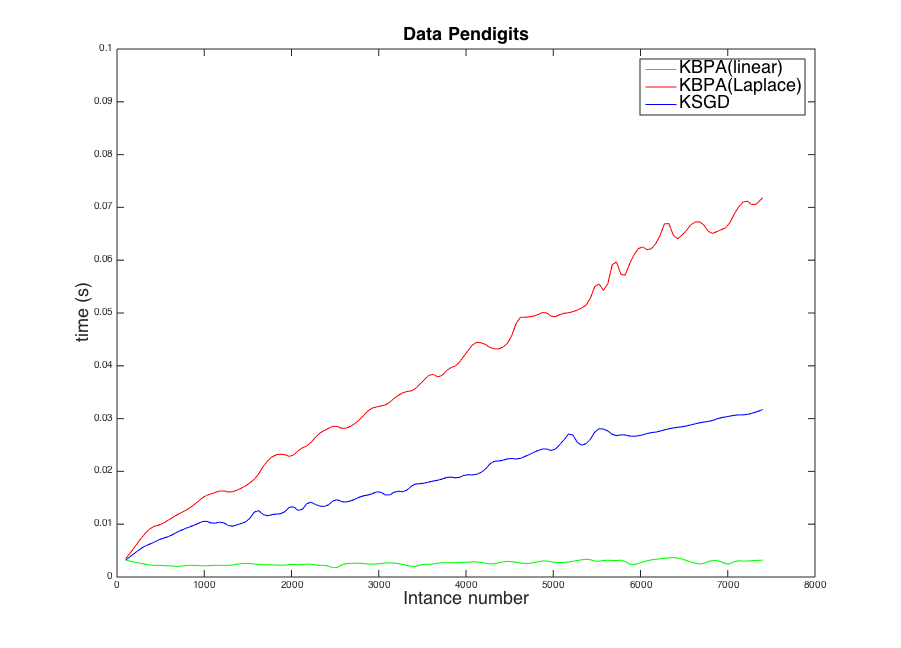
\includegraphics[scale = 0.4]{fig05/mc/Pendigits_kernel_T.png}
}
\caption{Average training time for each instance of Data Pendigits.}
\end{figure}

\begin{figure}[h!]
\label{pic:PKM}
\centerline{
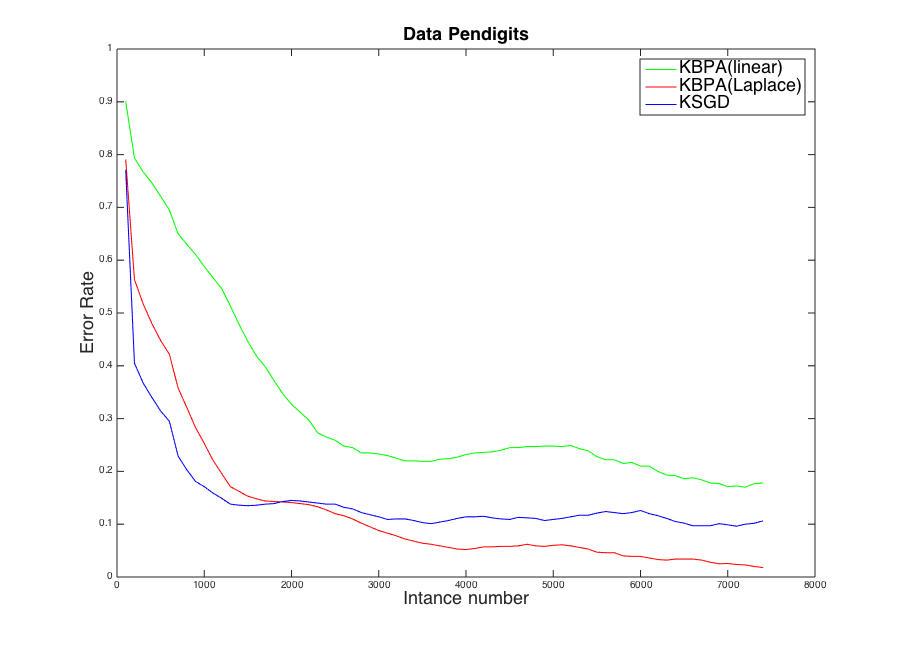
\includegraphics[scale = 0.4]{fig05/mc/Pendigits_kernel_M.png}}
\caption{Average error rate for each instance of Data Pendigits}
\end{figure}

\begin{figure}[h!]
\label{pic:PKCM}
\centerline{
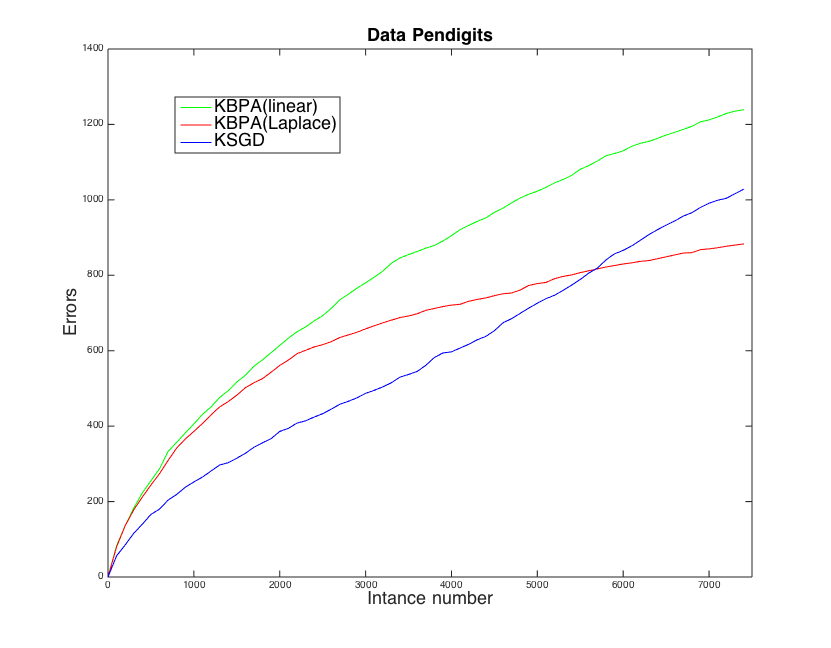
\includegraphics[scale = 0.4]{fig05/mc/Pendigits_kernel_CM.png}}
\caption{Cumulative Errors of Data Pendigits}
\end{figure}

\begin{figure}[h!]
\label{pic:PKR}
\centerline{
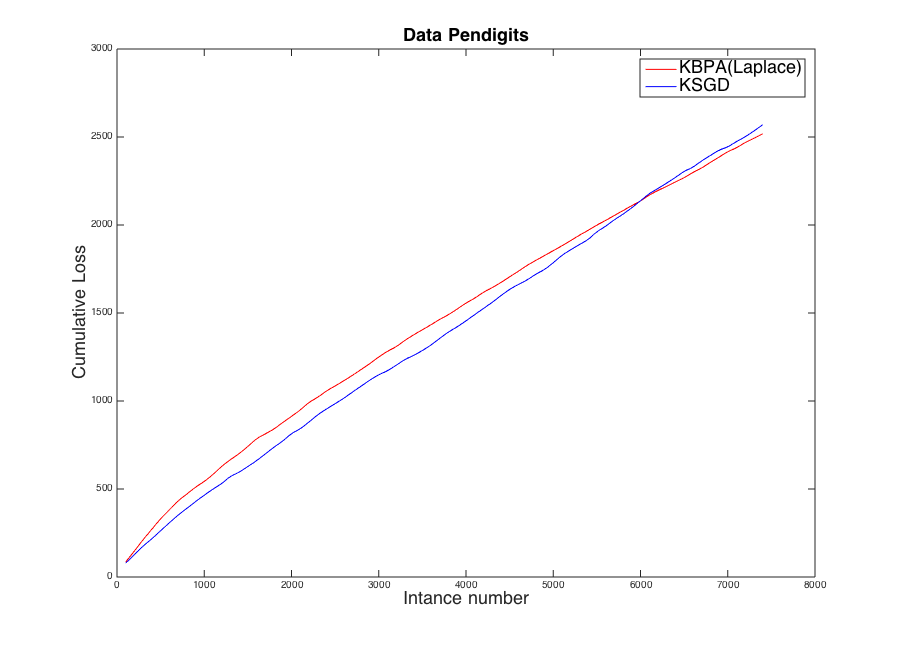
\includegraphics[scale = 0.4]{fig05/mc/Pendigits_kernel_R.png}}
\caption{Cumulative loss of Data Pendigits}
\end{figure}

\begin{figure}[h!]
\label{pic:SKT}
\centerline{
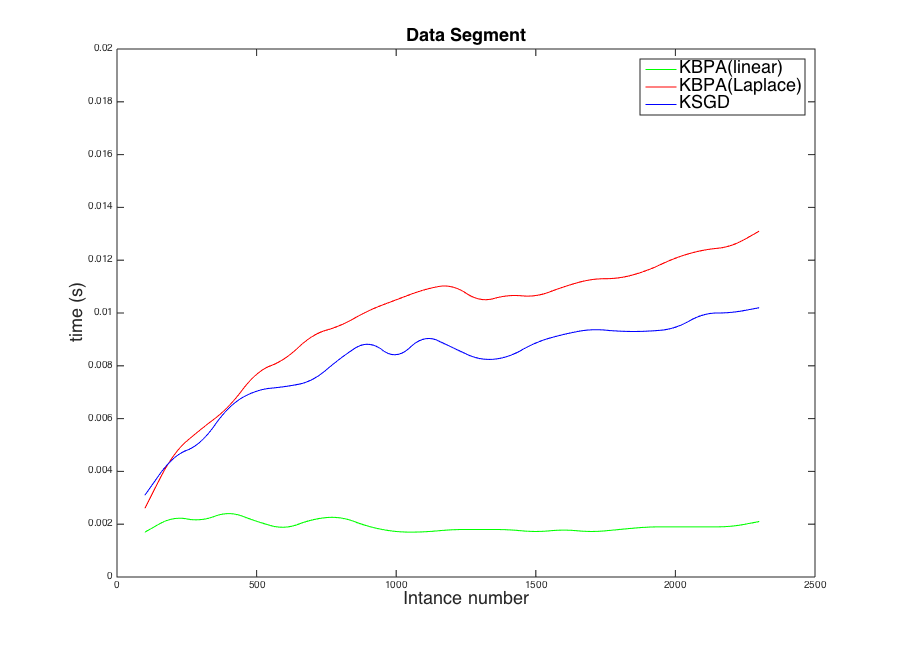
\includegraphics[scale = 0.4]{fig05/mc/Segment_kernel_T.png}}
\caption{Average training time for each instance of Data Segment.}
\end{figure}

\begin{figure}[h!]
\label{pic:SKM}
\centerline{
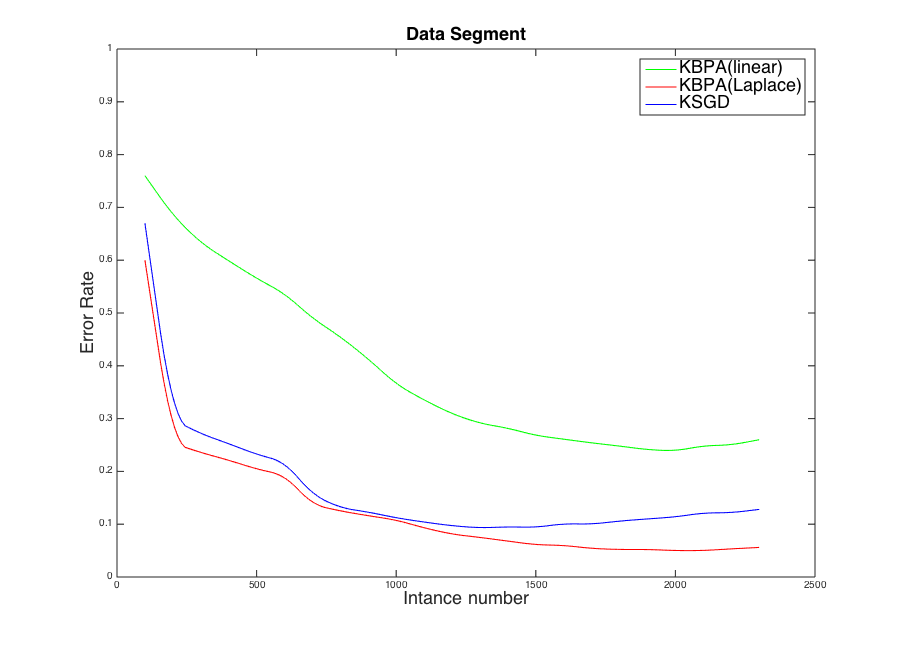
\includegraphics[scale = 0.4]{fig05/mc/Segment_kernel_M.png}}
\caption{Average error rate for each instance of Data Segment}
\end{figure}

\begin{figure}[h!]
\label{pic:SKCM}
\centerline{
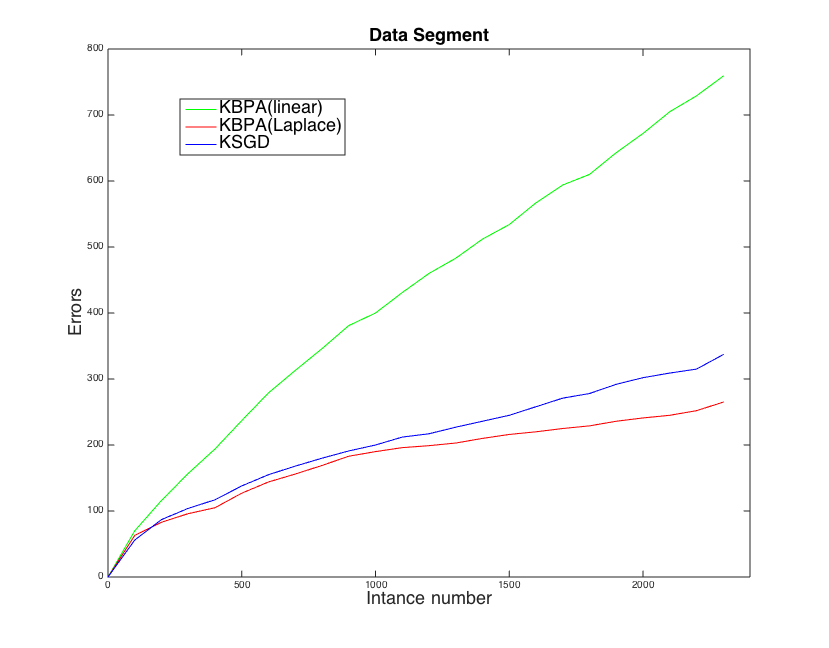
\includegraphics[scale = 0.4]{fig05/mc/Segment_kernel_CM.png}}
\caption{Cumulative Errors of Data Segment}
\end{figure}

\begin{figure}[h!]
\label{pic:SKR}
\centerline{
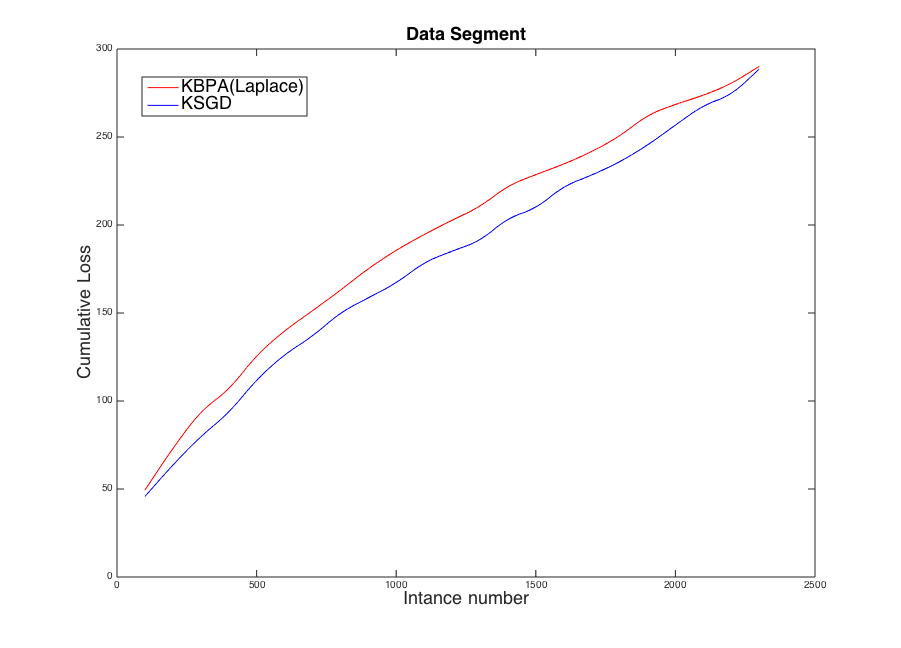
\includegraphics[scale = 0.4]{fig05/mc/Segment_kernel_R.png}}
\caption{Cumulative loss of Data Segment}
\end{figure}
\subsection{Conclusion}
